\section{Platform Architecture}
The system  is a comprehensive web-based healthcare management system developed to streamline medical services and enhance diagnostic workflows through an integrated digital platform. The system provides a centralized environment where patients, doctors, administrators, and healthcare institutions can interact efficiently through role-based dashboards and specialized services.
The platform allows patients to create accounts, manage their profiles, book appointments, track medical records, and communicate through an intelligent healthcare assistant. Doctors can manage appointments, analyze medical images, review patient information, and assign diagnostic results, while administrators oversee user management, system operations, and hospital coordination. The system also supports healthcare institutions participating in collaborative AI model development through federated learning mechanisms.
Built using a modern multi-tier architecture, XFed NeuroScan combines a responsive web interface, secure backend services, cloud-based storage, and artificial intelligence modules to deliver a seamless user experience. The application emphasizes security, scalability, and usability by implementing role-based access control, secure authentication, real-time communication, and centralized healthcare workflows.
By integrating healthcare management features with intelligent diagnostic services, XFed NeuroScan provides a unified platform that improves operational efficiency, supports medical decision-making, and enhances the overall experience for both healthcare providers and patients.

The platform is composed of four tightly integrated repositories:
\begin{itemize}
	\item \textbf{Frontend:} React 18 single-pages application serving doctors, patients, and administrators.
	\item \textbf{Backend:} Spring Boot 3.5 REST and WebSocket API acting as the central system of record, handling authentication, business logic, user management, and communication between services.
	\item \textbf{Model Backend:} FastAPI-based AI service responsible for medical image analysis, chest disease classification, lung cancer detection, explainable AI heatmap generation, and a Retrieval-Augmented Generation (RAG) medical chatbot for intelligent question answering.
	\item \textbf{Federated-Learning Server:} Flower-based federated learning coordinator managing hospital registration, client monitoring, distributed training rounds, and global model aggregation.
\end{itemize} 
Together, these components provide a complete healthcare platform that combines medical workflow management, AI-assisted diagnosis, intelligent medical assistance through RAG, and privacy-preserving federated learning across multiple healthcare institutions.

\begin{table}[htbp]
	\centering
	\caption{Summary of the proposed X-Fed NeuroScan framework.}
	\label{tab:framework_summary}
	\begin{tabular}{|p{4cm}|p{9cm}|}
		\hline
		\textbf{Dimension} & \textbf{Detail} \\
		\hline
		Primary Domain & Medical imaging and AI-based diagnostic systems \\
		\hline
		Key Innovation & Federated learning for privacy-preserving model improvement and collaborative model training across institutions \\
		\hline
		User Roles & Patient, Doctor, and Administrator \\
		\hline
		Imaging Modalities & Chest X-ray classification (COVID-19, Tuberculosis, Pneumonia, and Normal) and lung cancer detection from CT scans \\
		\hline
		AI Explainability & Grad-CAM heatmaps for chest disease predictions and lesion localization visualizations for lung cancer detection \\
		\hline
		Privacy Model & Raw medical images never leave hospital premises; only model parameters are exchanged during federated learning \\
		\hline
	\end{tabular}
\end{table}

\subsection{End-to-End System Architecture}The system follows a microservices architecture. Four independent services communicate over well-defined APIs. The frontend is the only entry point for human users; all backend services are internal.

\subsubsection{Service Map}
Table~\ref{tab:system_components} lists all the different components and services of the proposed system.
\begin{table}[htbp]
	\centering
	\caption{Technological components of the proposed system architecture.}
	\label{tab:system_components}
	\begin{tabular}{|p{3.5cm}|p{4.5cm}|p{2cm}|p{5cm}|}
		\hline
		\textbf{Service} & \textbf{Technology} & \textbf{Port} & \textbf{Primary Role} \\
		\hline
		Frontend &
		React 18, Vite, and TypeScript &
		3000 &
		User interface for patients, doctors, and administrators \\
		\hline
		
		Backend &
		Spring Boot 3.5 and Java 21 &
		8080 &
		Authentication, business logic implementation, and API gateway services \\
		\hline
		
		Model Backend &
		FastAPI and Python 3 &
		8000 &
		Machine learning inference services and retrieval-augmented generation (RAG) chatbot functionality \\
		\hline
		
		Federated Learning Server &
		FastAPI, Flower, and Python 3 &
		8001 / 50051 &
		Federated learning coordination, client management, and hospital registry services \\
		\hline
	\end{tabular}
\end{table}

\subsubsection{External Infrastructure}
During system implementation, we  have also relied on external components to not reinvent the wheel  and leverage already existing powerful and free infrastructure, those components are listed in Table~\ref{tab:supporting_infrastructure}
\begin{table}[htbp]
	\centering
	\caption{Supporting infrastructure and external services used by the proposed system.}
	\label{tab:supporting_infrastructure}
	\begin{tabular}{|p{4.5cm}|p{10cm}|}
		\hline
		\textbf{Component} & \textbf{Role} \\
		\hline
		
		Cloudflare R2 (S3-Compatible Storage) &
		Stores uploaded medical images, generated Grad-CAM heatmaps, lung cancer detection result overlays, and other imaging-related artifacts. \\
		\hline
		
		PostgreSQL &
		Primary relational database used to manage users, medical images, appointments, hospital information, federated learning participants, and other persistent application data. \\
		\hline
		
		Redis &
		Provides high-speed storage for refresh tokens and caching of presigned URLs to improve system performance and reduce unnecessary storage requests. \\
		\hline
		
		Ollama (qwen2.5:3b) &
		Local large language model (LLM) responsible for generating responses within the retrieval-augmented generation (RAG) chatbot component. \\
		\hline
		
		Gmail SMTP &
		Handles transactional email services including password reset requests, user invitations, account notifications, and hospital package communications. \\
		\hline
		
		FAISS &
		Vector similarity search engine used to index and retrieve relevant documents for the retrieval-augmented generation (RAG) pipeline. \\
		\hline
		
	\end{tabular}
\end{table}

\subsubsection{Architecture Visualization}

To provide a clearer understanding of the overall system structure, Figures~\ref{fig:system_architecture_overview} and \ref{fig:deployment_architecture_overview} present visual representations of the proposed \textit{X-Fed NeuroScan} framework. These diagrams complement the architectural descriptions presented throughout this chapter by illustrating the interaction between system components, data flow pathways, and deployment services. Together, they provide a comprehensive view of both the logical architecture of the framework and the technological infrastructure used to support its operation.

\begin{figure}[htbp]
	\centering
	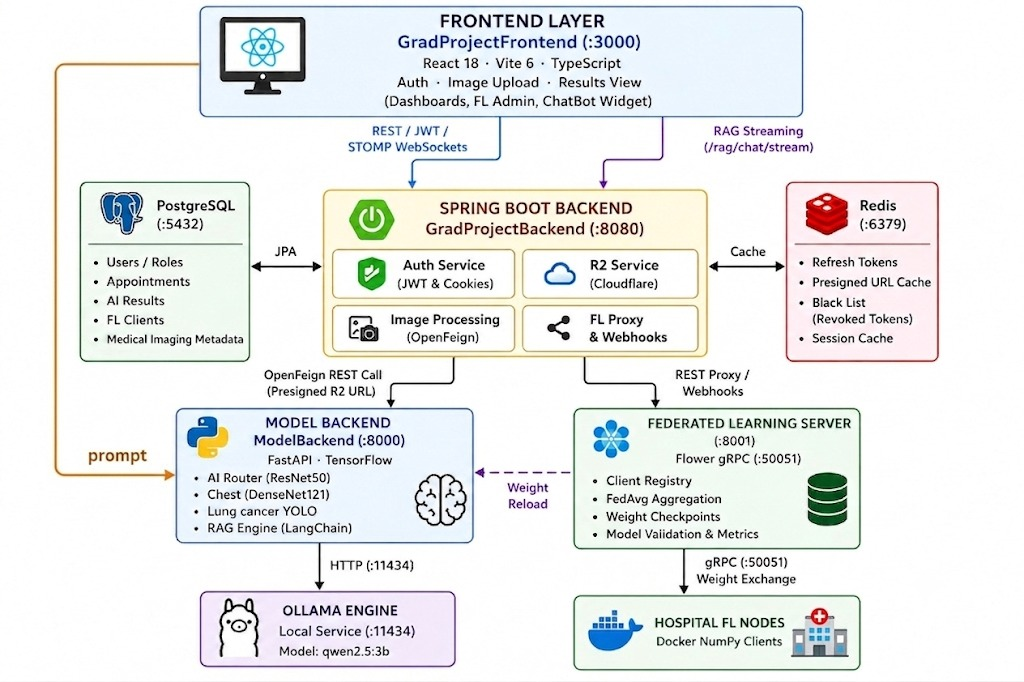
\includegraphics[width=0.95\linewidth]{assets/backend-1-ag.jpeg}
	\caption{End-to-end logical architecture of the proposed X-Fed NeuroScan framework, illustrating the interaction between users, backend services, AI models, explainability components, federated learning infrastructure, and data storage systems.}
	\label{fig:system_architecture_overview}
\end{figure}

\begin{figure}[htbp]
	\centering
	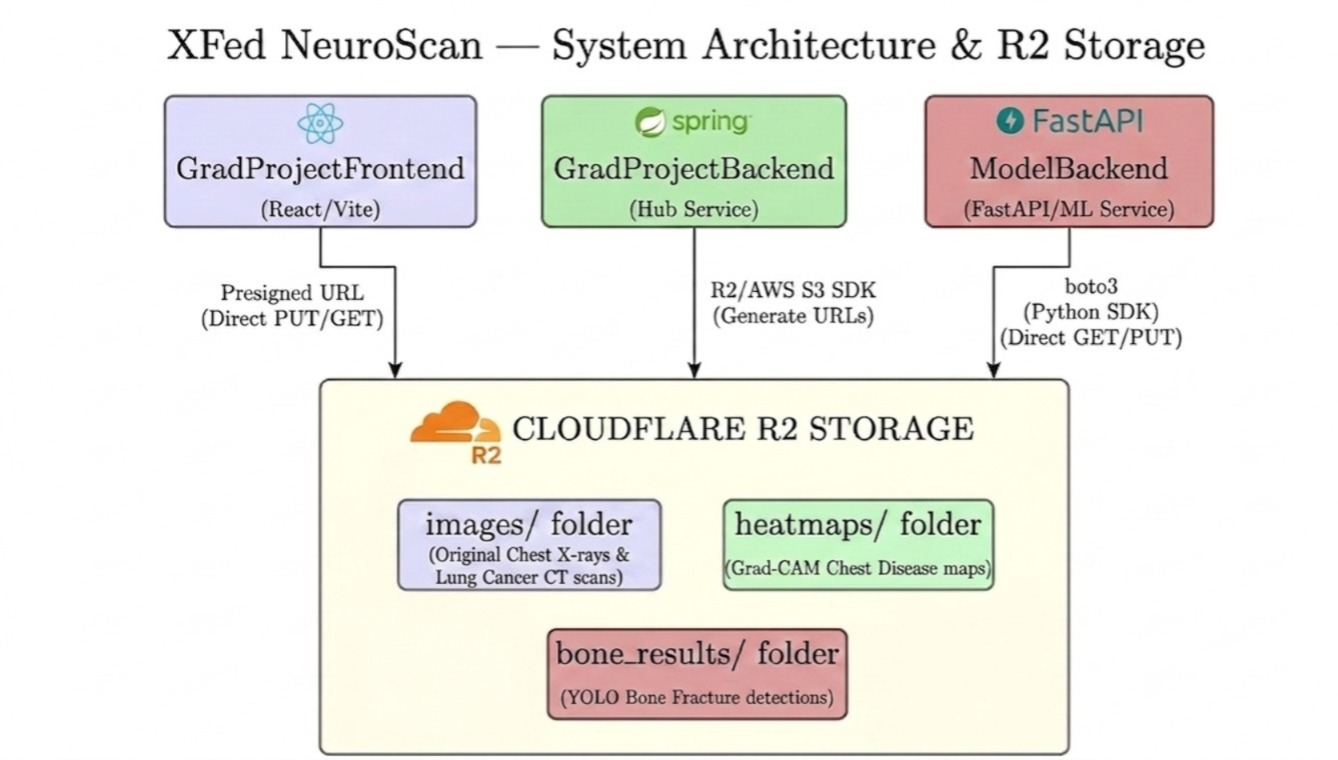
\includegraphics[width=0.95\linewidth]{assets/backend-2-ag.jpeg}
	\caption{Deployment architecture of the proposed system showing the frontend application, backend services, model-serving infrastructure, federated learning server, databases, storage components, and external integrations.}
	\label{fig:deployment_architecture_overview}
\end{figure}

\subsection{Frontend}
The frontend is a React 18 single-page application built with Vite 6 and TypeScript. It serves three user roles — Patient, Doctor, and Admin — through role-gated dashboards, and is the sole human interface into the platform.

\subsubsection{Technology Stack}
Different technologies were used during the development and implementation of the frontend components of the proposed system. They have been listed in Table~\ref{tab:frontend_technologies}.
\begin{table}[htbp]
	\centering
	\caption{Frontend technologies used in the implementation of the proposed system.}
	\label{tab:frontend_technologies}
	\begin{tabular}{|p{4cm}|p{8.5cm}|}
		\hline
		\textbf{Category} & \textbf{Technology} \\
		\hline
		
		Framework &
		React 18 \\
		\hline
		
		Build Tool &
		Vite 6 with \texttt{@vitejs/plugin-react-swc} \\
		\hline
		
		Programming Language &
		TypeScript 5 (Strict Mode) \\
		\hline
		
		Routing &
		React Router 7 \\
		\hline
		
		Styling &
		Tailwind CSS v4 \\
		\hline
		
		UI Primitives &
		Radix UI with shadcn-style wrapper components \\
		\hline
		
		Animations &
		Framer Motion (Motion) \\
		\hline
		
		Charts and Data Visualization &
		Recharts \\
		\hline
		
		Real-Time Communication &
		\texttt{@stomp/stompjs} and \texttt{sockjs-client} \\
		\hline
		
		Form Management &
		react-hook-form \\
		\hline
		
	\end{tabular}
\end{table}

\subsubsection{User Roles \& Capabilities}
The system is designed as a role-based healthcare to ensure that each type of user interacts with the platform according to their responsibilities, permissions, and level of access. The system defines three main roles: Patient, Doctor, and Administrator, each serving a distinct purpose within the healthcare workflow.

Patients represent the end users of the system. Their role is limited to personal healthcare management, including registering accounts, booking appointments, viewing medical history, and accessing their own diagnostic results. This restricted access ensures that patients can interact with their healthcare data securely without modifying clinical or system-level information.

Doctors have a more advanced role focused on medical operations. They can upload and analyze medical images, review AI-generated predictions, interpret results, and assign diagnoses to patients. In addition, doctors manage appointments and clinical interactions with patients. This role requires broader access because it directly involves medical decision-making and the use of AI diagnostic tools.
Administrators hold the highest level of control within the system. They are responsible for managing users, including creating and inviting doctors, monitoring system activity, and overseeing hospital and federated learning operations. Administrators also handle system configuration and ensure that all services operate securely and efficiently.

The separation of roles is essential for maintaining security, privacy, and operational clarity. By limiting access based on responsibilities, the system prevents unauthorized actions, reduces the risk of data misuse, and ensures that each user interacts only with the features relevant to their function. This role-based design also improves usability by providing a tailored interface for each type of user, making the system more efficient and easier to navigate.

\begin{table}[htbp]
	\centering
	\caption{User roles and capabilities within the proposed X-Fed NeuroScan system.}
	\label{tab:user_roles_capabilities}
	\begin{tabular}{|p{3cm}|p{9.5cm}|}
		\hline
		\textbf{Role} & \textbf{Capabilities} \\
		\hline
		
		Patient &
		View personalized dashboard statistics, book appointments with doctors, upload medical image attachments, access diagnostic results, and review prediction history. \\
		\hline
		
		Doctor &
		Analyze chest medical images using the integrated AI models, assign diagnostic results to patients, manage appointment schedules, review patient records, and access prediction history. \\
		\hline
		
		Administrator &
		Perform full platform administration including user management, federated learning hospital registration, hospital selection for federated training rounds, monitoring system activity, and conducting image analysis through the integrated diagnostic framework. \\
		\hline
		
	\end{tabular}
\end{table}

\subsubsection{Key Pages and Routing}
Frontend is structured as a single-page application with role-based routing to ensure secure and organized access to system features. Each user type is directed to specific pages depending on their permissions and responsibilities within the platform.

Public users can access the landing page and authentication-related pages, including login, signup, password recovery, and invite-based account activation. These pages are only available to guests who are not yet authenticated.

Authenticated users are redirected to role-specific dashboards after login. Patients have access to their personal dashboard and medical history, where they can view appointments and diagnostic results. Doctors are provided with a dedicated dashboard along with access to image analysis tools and patient-related medical data. Administrators have the highest level of access, allowing them to manage users, monitor system activity, and control federated learning operations.

In addition to dashboards, administrators also access specialized modules for user management and federated learning configuration, including hospital registration and training round setup. The image analysis page is restricted to doctors and administrators due to its clinical importance and use of AI-based diagnostic tools.

Overall, the routing structure enforces strict role-based access control, ensuring that each user interacts only with the features relevant to their responsibilities while maintaining system security and usability.

\begin{table}[htbp]
	\centering
	\caption{Access control policy for system pages and administrative modules.}
	\label{tab:system_page_access_control}
	\begin{tabular}{|p{4cm}|p{6.5cm}|}
		\hline
		\textbf{Page} & \textbf{Access} \\
		\hline
		
		Landing Page &
		Publicly accessible to all users, including unauthenticated visitors. \\
		\hline
		
		Authentication Pages &
		Accessible only to guest users who have not yet authenticated. \\
		\hline
		
		Password Recovery &
		Accessible only to guest users initiating the password reset process. \\
		\hline
		
		Invite Activation &
		Accessible only through a valid invitation token provided to the invited user. \\
		\hline
		
		Image Analysis &
		Accessible to users with Administrator or Doctor privileges. \\
		\hline
		
		Prediction History &
		Accessible to Administrators, Doctors, and Patients according to their authorization level. \\
		\hline
		
		Administrator Dashboard &
		Accessible exclusively to users with the Administrator role. \\
		\hline
		
		Doctor Dashboard &
		Accessible exclusively to users with the Doctor role. \\
		\hline
		
		Patient Dashboard &
		Accessible exclusively to users with the Patient role. \\
		\hline
		
		User Management &
		Accessible exclusively to Administrators for managing user accounts and permissions. \\
		\hline
		
		Federated Learning Hospital Management &
		Accessible exclusively to Administrators for registering, updating, and monitoring participating hospitals. \\
		\hline
		
		Federated Learning Training Round Setup &
		Accessible exclusively to Administrators for configuring and launching federated learning training rounds. \\
		\hline
		
	\end{tabular}
\end{table}

\subsubsection{Core Features}
\paragraph{Authentication \& Session Management}
The frontend implements a full authentication lifecycle using JWT access tokens are stored in memory (not localStorage); refresh tokens are stored in HttpOnly cookies. On app load, the context attempts a silent token refresh to restore sessions without requiring re-login. GuestRoute prevents authenticated users from visiting auth. pages; Require Dashboard Role guards all dashboard routes.

\paragraph{Medical Image Analysis}
The image analysis flow uses a presigned-URL pattern to avoid routing large files through the backend:
\begin{itemize}
	\item Step 1: Frontend requests a presigned R2 PUT URL from Spring Backend 
	\item Step 2: Frontend uploads the image directly to Cloudflare R2
	\item Step 3: Frontend calls the api who is responsible for image-processing with the R2 key
	\item Step 4: Backend triggers Model inference and returns prediction, confidence, and heatmap URL
\end{itemize}

\paragraph{Federated Learning Management}
Admins manage FL hospitals through two dedicated pages. FLHospitalsPage shows all registered hospital nodes with live ONLINE/OFFLINE status via WebSocket. FL Select Hospitals Page lets admins choose which hospitals participate in the next training round. Registration generates an API key displayed once via ApiKeySuccessDialog.

\paragraph{AI Chatbot (RAG)}
A floating chat widget  is available on every page. Responses are streamed from the RAG service. The chatbot gracefully degrades to keyword-based mock answers if the RAG API is unreachable.

\begin{figure}[htbp]
	\centering
	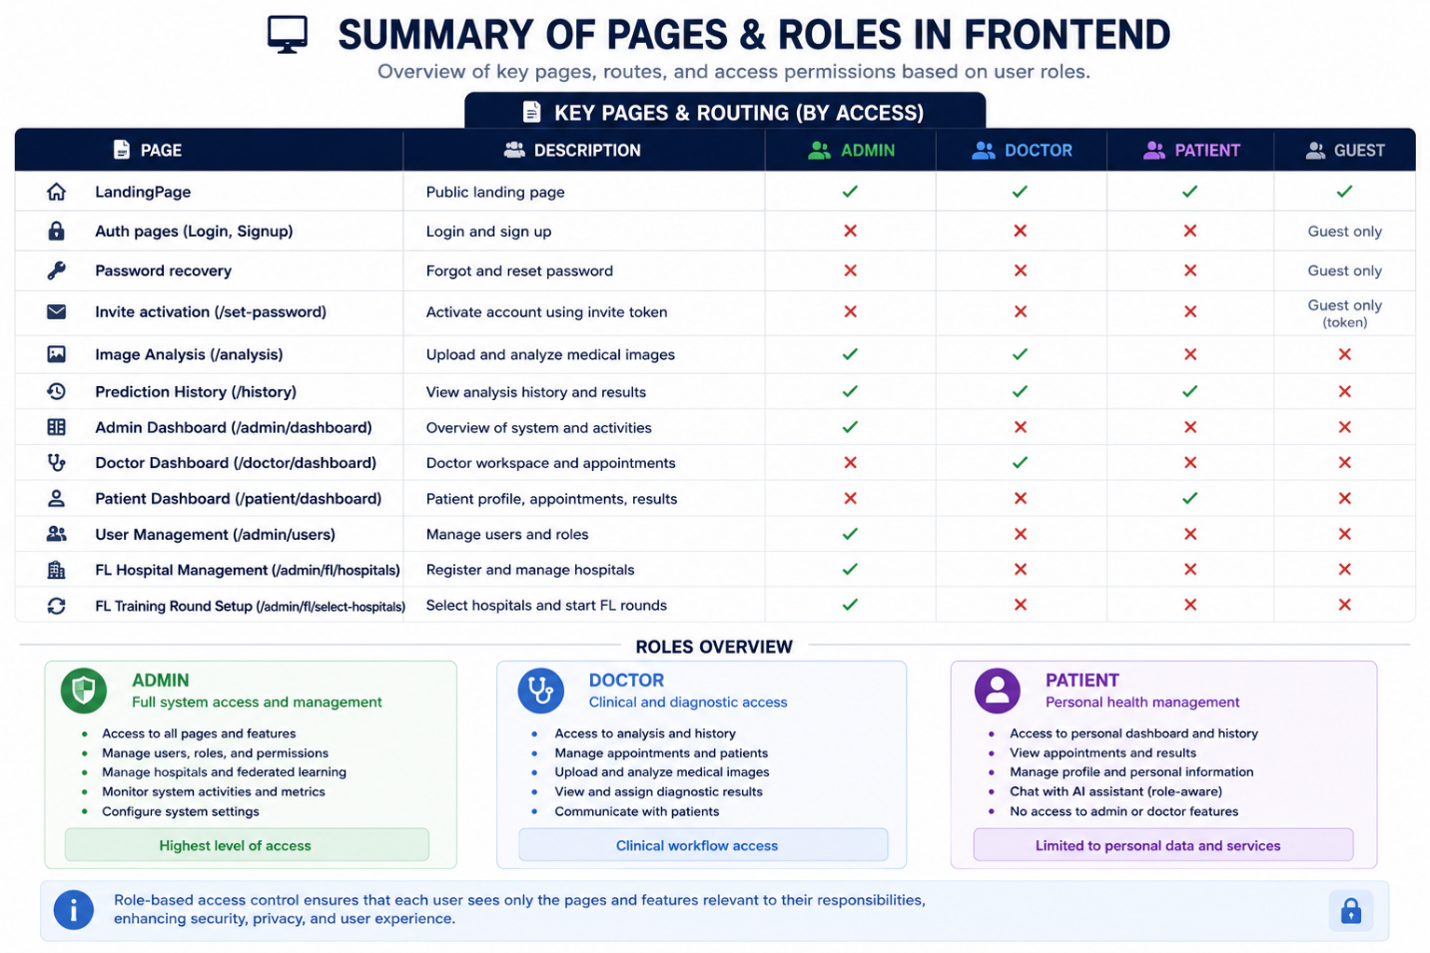
\includegraphics[width=0.95\linewidth]{assets/backend3.png}
	\caption{A visualization of the roles and pages implemented in the web application.}
	\label{fig:roles_pages_summary}
\end{figure}

\subsection{Centralized Backend (Spring Boot)}
Centralized backend is a Spring Boot 3.5 application written in Java 21. It serves as the central API gateway and system of record for authentication, user management, medical image orchestration, appointments, federated learning coordination, and real-time WebSocket broadcasts. 

\subsubsection{Technology Stack}
Various technologies were utilized in the implementation of the backend of the proposed end-to-end system. All of these technologies are listed in Table~\ref{tab:backend_technologies}.
\begin{table}[htbp]
	\centering
	\caption{Backend technologies used in the implementation of the proposed system.}
	\label{tab:backend_technologies}
	\begin{tabular}{|p{4cm}|p{8.5cm}|}
		\hline
		\textbf{Category} & \textbf{Technology} \\
		\hline
		
		Framework &
		Spring Boot 3.5.4 \\
		\hline
		
		Programming Language &
		Java 21 \\
		\hline
		
		Build Tool &
		Maven \\
		\hline
		
		Security &
		Spring Security 6 with JSON Web Token (JWT) authentication using JJWT 0.12.3 \\
		\hline
		
		Persistence Layer &
		Spring Data JPA, Hibernate, and PostgreSQL \\
		\hline
		
		Cache and Session Management &
		Spring Data Redis \\
		\hline
		
		HTTP Client &
		Spring Cloud OpenFeign \\
		\hline
		
		Real-Time Communication &
		Spring WebSocket, STOMP, and SockJS \\
		\hline
		
		Object Storage Integration &
		AWS SDK v2 for S3-compatible storage (Cloudflare R2) \\
		\hline
		
		Email Services &
		Spring Mail with Gmail SMTP \\
		\hline
		
		API Documentation &
		SpringDoc OpenAPI (Swagger UI) \\
		\hline
		
		Object Mapping and Code Generation &
		MapStruct and Lombok \\
		\hline
		
	\end{tabular}
\end{table}

\subsubsection{Security \& Authentication}

\begin{figure}[htbp]
	\centering
	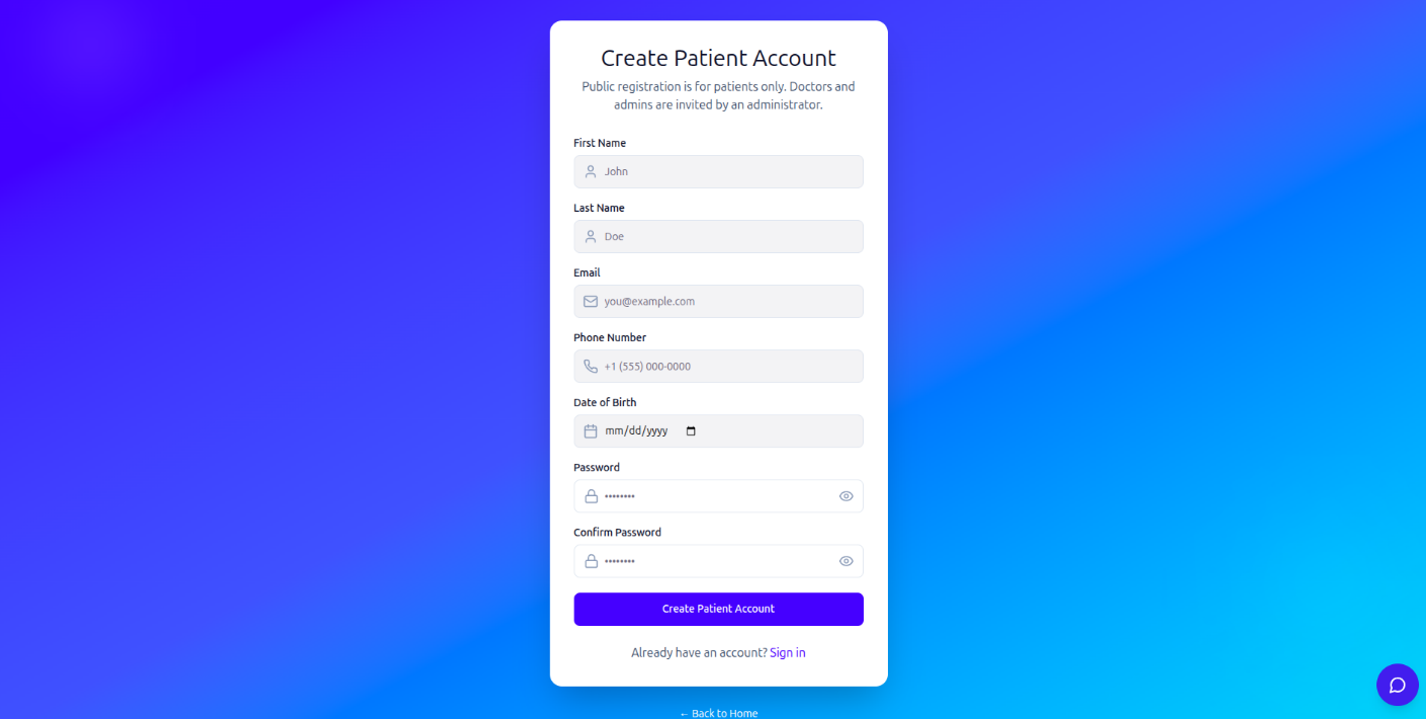
\includegraphics{assets/backend4.png}
	\caption{An image of the Create Account interaction from the web application.}
	\label{fig:create_account}
\end{figure}

\begin{figure}[htbp]
	\centering
	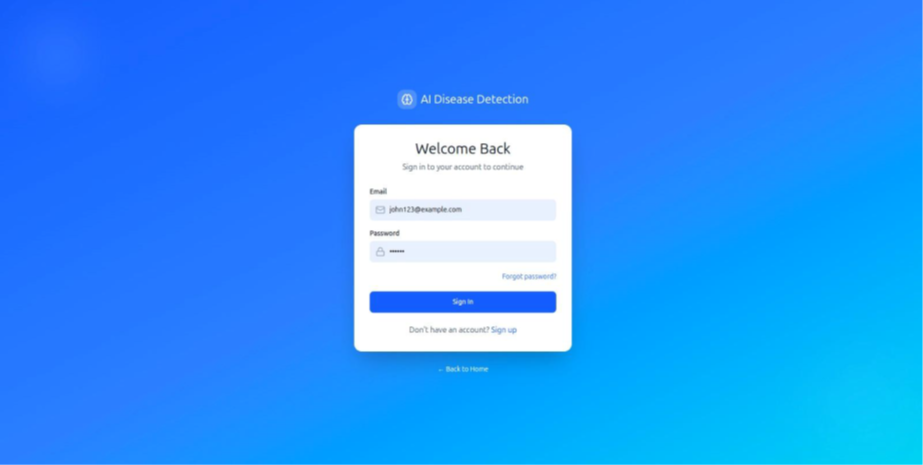
\includegraphics{assets/backend5.png}
	\caption{An image of the Login interaction from the web application.}
	\label{fig:login}
\end{figure}

Security is implemented with JWT access tokens and HttpOnly refresh-token cookies stored in Redis:
\begin{itemize}
	\item Access Tokens: short-lived JWTs returned in the login response body
	\item Refresh Tokens: longer-lived tokens stored in Redis (key: email:deviceId) and set as HttpOnly cookies
	\item Logout: access tokens blacklisted when still valid; refresh token deleted from Redis
	\item FL API keys: encrypted at rest using AES via EncryptionUtils
	\item FL webhook endpoints: authenticated with a shared secret (not JWT)
	\item Soft delete: deleted users cannot log in
\end{itemize}

In the current system design, \textbf{login is restricted to patients only}. Doctor and Admin accounts are not self-authenticated through public signup; instead, they are created and managed exclusively by an administrator and activated through an invitation-based workflow. This ensures strict control over privileged roles in the healthcare system.

After login, user information is stored in PostgreSQL, but sensitive session data is handled separately for security. Passwords are never stored in plain text; instead, they are hashed using \textbf{BCrypt} before being saved in the database, making them irreversible and protected even if the database is compromised.

During authentication, the input password is hashed and compared with the stored hash. If valid, the system generates a short-lived \textbf{JWT access token} and a long-lived \textbf{refresh token}. The access token is used for API requests, while the refresh token is stored securely in \textbf{Redis} and also set as an \textbf{HttpOnly cookie}.

When the user logs out, the access token is blacklisted and the refresh token is removed from Redis, fully terminating the session. This design ensures secure password storage, stateless authentication, and strong session protection. 

In the system, only Admin users have the authority to create or manage Doctor and other Admin accounts, ensuring strict role control and preventing unauthorized privilege escalation.

New privileged users (Doctors or Admins) cannot register through the public signup process. Instead, an Admin must explicitly create or invite them through the administrative interface. This invitation-based flow allows the system to maintain tight control over sensitive roles that have access to clinical data, AI analysis tools, and system-wide management features.

\begin{figure}[htbp]
	\centering
	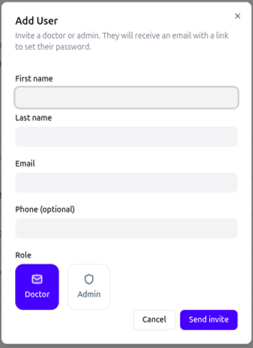
\includegraphics{assets/backend6.png}
	\caption{An image of the Add User interaction from the web application.}
	\label{fig:add_user}
\end{figure}

After an Admin creates a new Doctor or Admin account, the account does not become active immediately. Instead, it enters a pending state until it is explicitly approved. This approval step ensures that no privileged user gains access to the system without proper verification and administrative confirmation.

During this pending phase, the user record is already stored in the database, but the account remains inactive, meaning the user cannot log in or access any system features. Once the Admin approves the account, its status is updated to active, and the user is then able to authenticate and use the system according to their assigned role.

In the user management interface, the Admin has full control over viewing and organizing all system users through a role-based filtering system. This allows the Admin to efficiently manage large numbers of accounts by categorizing users according to their current role and status.

In addition to account creation and approval, the Admin also has full control over existing privileged accounts, as shown in \ref{fig:user_mgmt}. This includes the ability to disable or delete accounts at any time. Disabling an account temporarily prevents the user from logging in without removing their data, while deletion marks the account as removed (soft delete), ensuring it is excluded from authentication and system operations but still preserved for audit or historical purposes.

\begin{figure}[htbp]
	\centering
	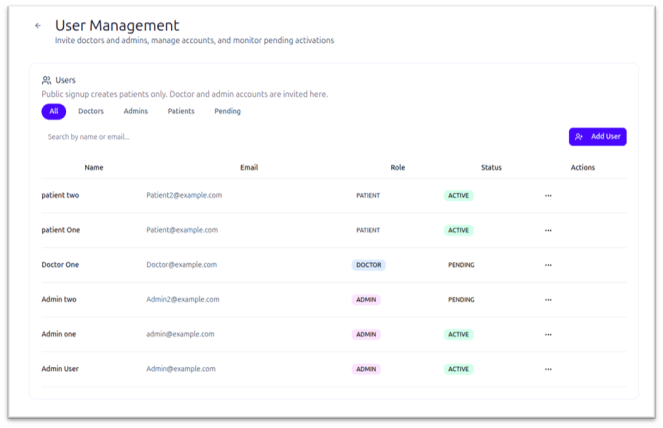
\includegraphics[width=0.95\linewidth]{assets/backend7.png}
	\caption{An image of the User Management tab from the web application.}
	\label{fig:user_mgmt}
\end{figure}

When a user selects “Forgot Password”, the system follows a secure multi-step flow to ensure that only the legitimate account owner can reset the password.

First, the user enters their registered email address in the frontend. This request is sent to the Spring Boot backend, which validates whether the email exists in the system. If the user is found, Spring Boot generates a secure password reset token, typically a short-lived, random token linked to the user account.

This token is then stored temporarily (or associated with the user record) and sent to the user via email using Gmail SMTP. The email contains a secure reset link that includes the token as a parameter.

When the user clicks the link, they are redirected to the password reset page in the frontend. The new password is submitted along with the token, and Spring Boot validates the token to ensure it is still valid and has not expired or been used before.

If the token is valid, the system hashes the new password using BCrypt and updates it in the PostgreSQL database, replacing the old password hash. After successful reset, the token is invalidated to prevent reuse.

Overall, the forgot password process ensures security by combining email verification, time-limited tokens, secure transmission, and encrypted password storage.

So in summary User authentication in system uses a secure JWT-based system where only patients can self-register and log in, while doctors and admins are created by admins. Passwords are stored in the database using BCrypt hashing.

After successful login, the system issues a short-lived JWT access token and a long-lived refresh token stored in Redis as an HttpOnly cookie. The access token is used for requests, and the refresh token allows session renewal.

The system also supports a secure forgot password workflow, where a password reset token is generated, sent to the user via email, and validated before allowing password updates. The new password is then hashed using BCrypt and stored in the database.

On logout, tokens are invalidated by blacklisting the access token and removing the refresh token. Role-based access control and soft delete ensure only authorized and active users can access the system.

\begin{figure}[htbp]
	\centering
	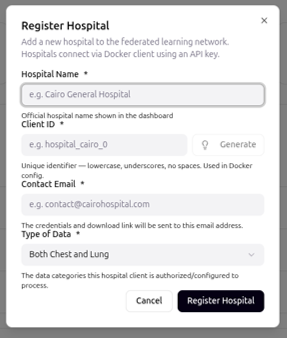
\includegraphics{assets/backend8.png}
	\caption{An image of the Add Hospital interaction from the web application.}
	\label{fig:add_hospital}
\end{figure}

\begin{figure}[htbp]
	\centering
	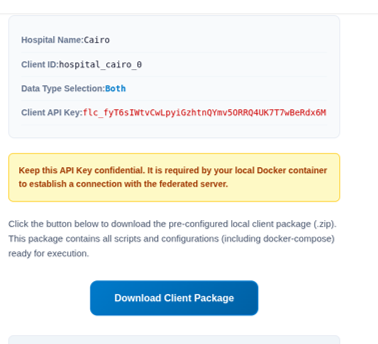
\includegraphics{assets/backend9.png}
	\caption{An image of the client hospital getting a confidential API key interaction from the web application.}
	\label{fig:hospital_api}
\end{figure}

Backend handles the full lifecycle of registering new hospitals in the federated learning system. When an Admin submits a hospital, Spring Boot validates the request, ensures only Admins can perform the action, and then generates a unique FL client ID and encrypted API key using AES before storing them in PostgreSQL. The hospital is initially saved with a PENDING or INACTIVE status.

After that, Spring Boot registers the hospital with the Federated Learning Server by sending its credentials and metadata, allowing it to join the federated learning network. It may also provide a Docker-based client package for hospital deployment.

Spring Boot receives and synchronizes key data from the Federated Learning (FL) Server, especially hospital online/offline status, which is determined by heartbeat signals sent from hospital clients to the FL Server. Spring Boot does not calculate this status itself; instead, it periodically fetches updated client information from the FL Server.

Overall, Spring Boot acts as a bridge that collects, stores, and distributes FL Server status updates, giving administrators a live view of the federated learning network.

When a new hospital is registered in the federated learning system, Spring Boot not only creates and stores the hospital record, but also sends an automated email notification via Gmail SMTP as part of the onboarding process.

After the Admin submits and approves the hospital registration, Spring Boot generates the hospital’s federated learning credentials (such as the FL client ID and encrypted API key) and securely stores them in the database. Once the registration is successfully completed, Spring Boot triggers the email service to notify the hospital.

This email is sent using Gmail SMTP integration and typically contains important onboarding information such as the hospital’s activation status, instructions for joining the federated learning network, and in some cases, a link or attachment for downloading the Docker-based FL client package required to connect to the FL server.

This step ensures that hospitals are immediately informed after registration and can proceed with setup and participation in federated learning without manual coordination. It also improves system automation and reduces administrative overhead while maintaining secure delivery of sensitive setup information.

\subsubsection{Medical Image Pipeline}
The backend orchestrates image analysis without storing raw images locally:
\begin{itemize}
	\item Presigned PUT URL is generated for direct R2 upload (5-minute expiry).
	\item After upload, backend saves image metadata to PostgreSQL
	\item ModelBackend is called via OpenFeign (Feign client) with a presigned GET URL
	\item ML results — prediction label, confidence score, heatmap S3 key — are persisted
	\item Presigned GET URLs for original and heatmap images are cached in Redis (~59 min TTL)
\end{itemize}

Small parts of the pipeline can be shown in \ref{fig:greeting_}, and \ref{fig:greeting_2} where the user is asked to upload a medical image to the system so that they are directed to the right models and diagnosed.

\begin{figure}[htbp]
	\centering
	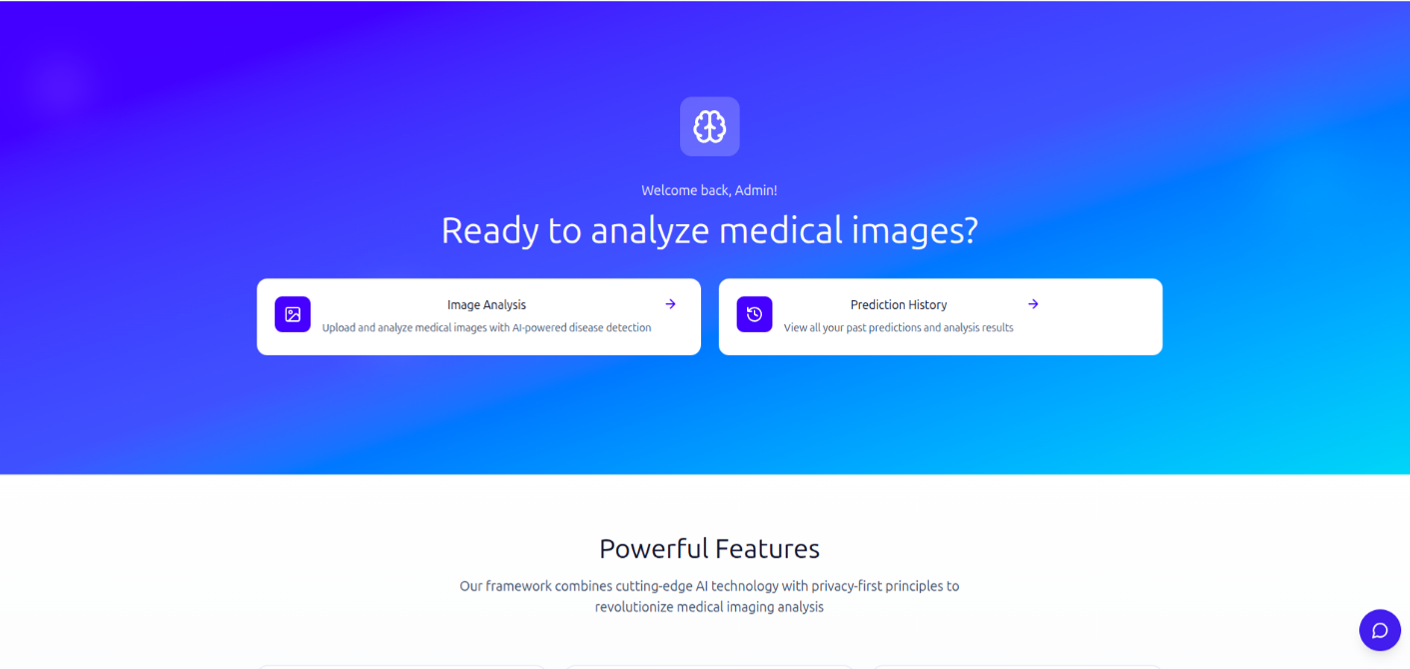
\includegraphics[width=0.95\linewidth]{assets/backend10.png}
	\caption{An image greeting page of the web application.}
	\label{fig:greeting_1}
\end{figure}

\begin{figure}[htbp]
	\centering
	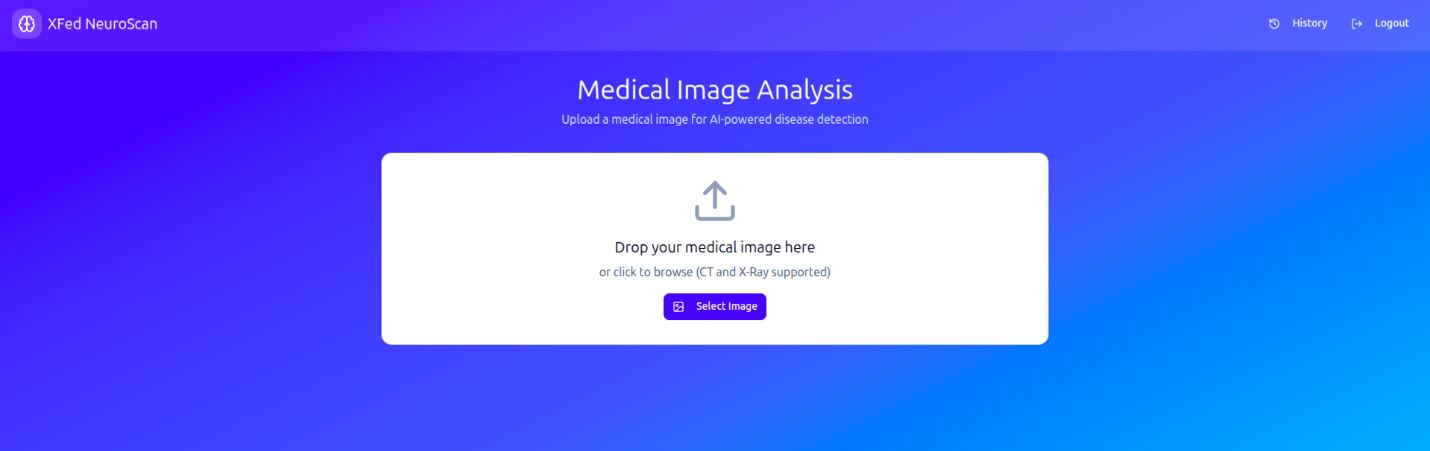
\includegraphics[width=0.95\linewidth]{assets/backend11.png}
	\caption{An image of the system asking the user to upload a scan to diagnose.}
	\label{fig:greeting_2}
\end{figure}

Prediction history can be viewed and also has statistics like (total scans , AVG. confidence) , and also every prediction’s details can be viewed or deleted, as shown in Figure~\ref{fig:pred_history}, and the details of each scan can be reviewed as well, as shown in Figure~\ref{fig:pred_review}.

\begin{figure}[htbp]
	\centering
	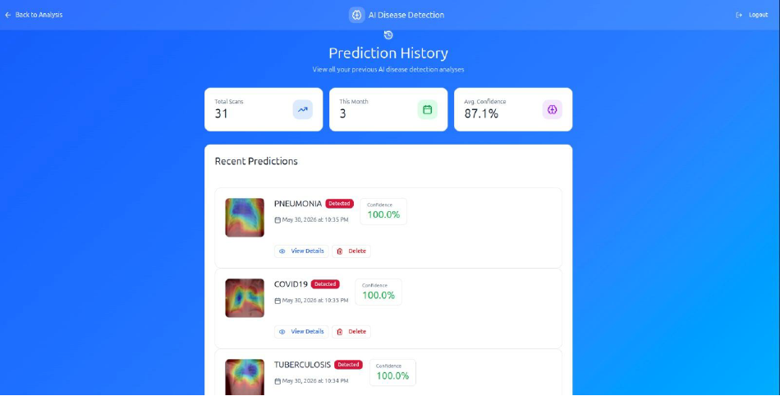
\includegraphics[width=0.95\linewidth]{assets/backend12.png}
	\caption{An image of the system showing the prediction history of the logged-in  user.}
	\label{fig:pred_history}
\end{figure}

\begin{figure}[htbp]
	\centering
	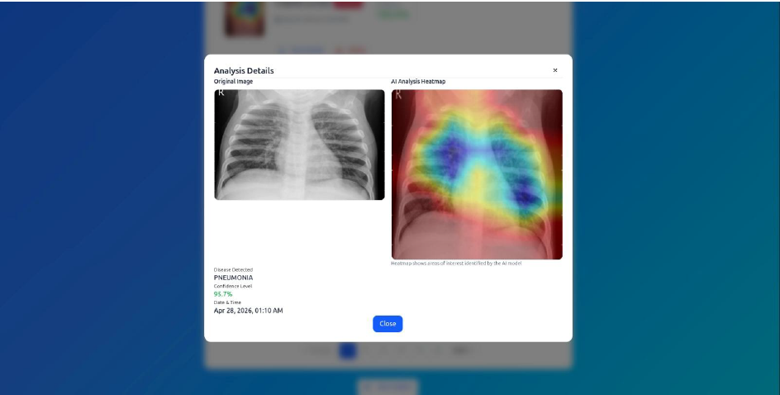
\includegraphics[width=0.95\linewidth]{assets/backend13.png}
	\caption{An image of the system showing the details of one of the user's historical predictions.}
	\label{fig:pred_review}
\end{figure}

Some examples of the Lung Cancer model in action are shown in Figure~\ref{fig:lung1}, and Figure~\ref{fig:lung2}. The system also makes sure to show the confidence as ordinary in medical applications of computer vision systems, as well as the processing time and the resulting heatmap, if applicable.

\begin{figure}[htbp]
	\centering
	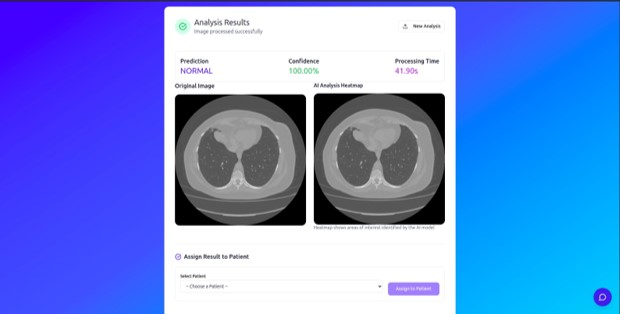
\includegraphics[width=0.95\linewidth]{assets/backend14.jpg}
	\caption{One of the of the examples of using the system on the a lung cancer image.}
	\label{fig:lung1}
\end{figure}

\begin{figure}[htbp]
	\centering
	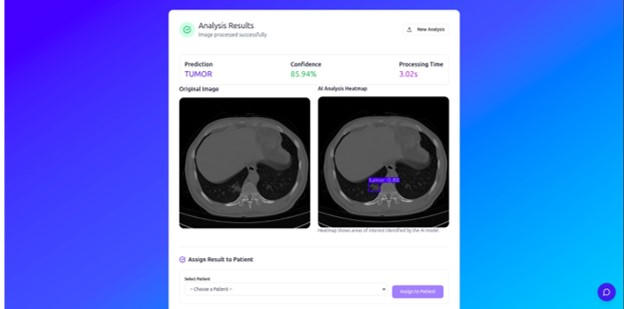
\includegraphics[width=0.95\linewidth]{assets/backend15.jpg}
	\caption{Another example of using the system on the a lung cancer image.}
	\label{fig:lung2}
\end{figure}

\subsubsection{Appointment Management}
The appointment management module enables patients and doctors to coordinate medical consultations through a structured workflow. Patients can create appointments by selecting a doctor, choosing a date and time, specifying the appointment type, and providing optional notes or supporting attachments. Once submitted, the appointment information is stored in the database and becomes available to the assigned doctor.

Doctors can view their scheduled appointments, review patient details, and update the appointment status as needed. They can mark appointments as completed, add consultation notes, or cancel appointments when necessary. Patients can also view the status of their appointments and track any updates made by the doctor.

All appointment data is managed through the Spring Boot backend and stored in PostgreSQL, ensuring persistence and secure access. The module provides an organized way to manage patient-doctor interactions while maintaining a complete record of appointment history within the platform.

\begin{figure}[htbp]
	\centering
	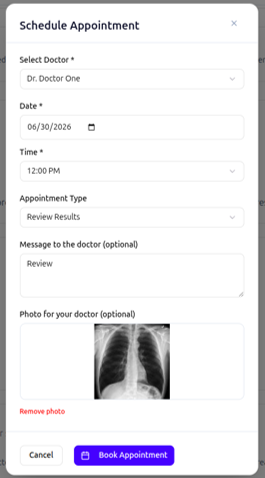
\includegraphics{assets/backend16.png}
	\caption{An image of the Schedule Appointment interaction from the system.}
	\label{fig:appointment_mgmt}
\end{figure}

\paragraph{Real-Time WebSocket}
Spring WebSocket with STOMP over SockJS provides live FL hospital status to the frontend. A scheduled poller runs every 10 seconds, fetches client status from the FL Server, syncs to PostgreSQL, and broadcasts to /topic/fl/clients. Hospital nodes that miss heartbeats are marked OFFLINE automatically.

\paragraph{Email Service}
Spring Mail with Gmail SMTP sends three types of emails:
\begin{itemize}
	\item Password Reset: link to \texttt{/reset-password?token=...}
	\item Admin Invite: link to \texttt{/set-password?token=...} for new doctor/admin accounts
	\item FL hospital onboarding: download link for the hospital Docker client package plus connection details.
\end{itemize}

\paragraph{Core API Modules}
The core modules exposed by the API and implemented in it a re listed in Table~\ref{tab:backend_modules}
\begin{table}[htbp]
	\centering
	\caption{Backend service modules and their responsibilities within the system.}
	\label{tab:backend_modules}
	\begin{tabular}{|p{4cm}|p{9cm}|}
		\hline
		\textbf{Module} & \textbf{Description} \\
		\hline
		
		Authentication &
		Handles the full authentication lifecycle including user registration, login, token issuance, refresh token management, and logout operations. \\
		\hline
		
		Image Upload &
		Generates and returns Cloudflare R2 presigned PUT URLs to enable secure direct client-side uploads of medical images. \\
		\hline
		
		Image Processing &
		Orchestrates the machine learning inference pipeline, triggers model execution, and stores as well as retrieves diagnostic results from the persistence layer. \\
		\hline
		
		Appointments &
		Manages the full appointment workflow, allowing patients to book appointments and doctors to approve, complete, or cancel scheduled sessions. \\
		\hline
		
		Admin User Management &
		Provides administrative capabilities for managing user accounts, including creation, modification, role assignment, and deactivation. \\
		\hline
		
		Federated Learning Hospitals &
		Handles hospital registration and management within the federated learning ecosystem, acting as a proxy interface to the federated learning server. \\
		\hline
		
		Federated Learning Webhooks &
		Processes callback events from the federated learning server after training rounds, updating system state and storing training metadata accordingly. \\
		\hline
		
	\end{tabular}
\end{table}

\subsection{ML Service - ModelBackend}
ModelBackend is a FastAPI microservice that hosts all AI capabilities. At startup it loads four ML components into memory and exposes a unified image-processing endpoint plus a RAG chatbot. It runs on port 8000 and is called by centralized Backend for image analysis and directly by the frontend for chatbot interactions.

\subsubsection{ML Models}
Different backbone models were used for the different tasks the proposed system performs. All the AI models and architectures used are listed in Table~\ref{tab:ml_components}.

\begin{table}[htbp]
	\centering
	\caption{Machine learning components and their corresponding frameworks and purposes within the proposed system.}
	\label{tab:ml_components}
	\begin{tabular}{|p{4cm}|p{5cm}|p{6cm}|}
		\hline
		\textbf{Component} & \textbf{Framework} & \textbf{Purpose} \\
		\hline
		
		Router Model &
		Keras (DenseNet121) &
		Classifies input images into X-ray, CT scan, or out-of-distribution categories using 224×224 image resolution as the first stage of the diagnostic pipeline. \\
		\hline
		
		Chest Classification &
		TensorFlow/Keras (DenseNet121) &
		Performs four-class chest X-ray diagnosis including COVID-19, Normal, Pneumonia, and Tuberculosis classification in a multi-label-ready setup. \\
		\hline
		
		Lung Segmentation &
		TensorFlow/Keras (U-Net) &
		Extracts lung regions from medical images prior to classification to enhance focus on relevant anatomical structures and improve diagnostic accuracy. \\
		\hline
		
		Lung Cancer Detection &
		YOLOv8 &
		Detects and localizes lung cancer regions in CT scans using bounding box predictions for object-level medical diagnosis. \\
		\hline
		
		RAG Stack &
		LangChain, Ollama, and FAISS &
		Implements a retrieval-augmented generation chatbot for medical question answering using vector-based document retrieval and local LLM inference. \\
		\hline
		
	\end{tabular}
\end{table}

FastAPI serves as the AI engine of XFed NeuroScan and relies on Spring Boot to integrate its models into the complete healthcare platform. While FastAPI is responsible for running AI models and generating predictions, Spring Boot manages the workflow and communicates with the AI service whenever analysis is requested.

Separating Spring Boot and FastAPI into two services improves scalability and maintainability, allowing the healthcare system and AI models to be developed, updated, and deployed independently without affecting each other.

\subsubsection{Image Processing Pipeline}
The image processing module is designed to automatically analyze uploaded medical images and route them to the appropriate AI model based on their content. This architecture allows the system to support multiple diagnostic pipelines while maintaining a single entry point for image analysis.

\paragraph{Unified Routing}
Every uploaded image first passes through the Router Model, which serves as the initial classification layer. The router determines whether the image is a chest X-ray, lung cancer image, or an unsupported image type. A confidence threshold of 0.5 is used to ensure reliable routing decisions. Images classified as other are immediately rejected to prevent invalid data from being processed by diagnostic models. Once classified, chest X-rays are forwarded to the DenseNet-based chest disease pipeline, while lung cancer images are sent to the YOLOv8 detection pipeline.

\paragraph{Chest Pipeline}
The chest disease analysis pipeline is optimized for detecting four classes: COVID-19, Pneumonia, Tuberculosis, and Normal. Before classification, several preprocessing steps are applied to improve image quality and model performance.

First, a U-Net lung segmentation model isolates the lung region from the surrounding anatomy, allowing the classifier to focus only on clinically relevant areas. Next, Contrast Limited Adaptive Histogram Equalization (CLAHE) enhances local contrast within the segmented lungs, making subtle abnormalities easier to detect. A Gaussian Blur (5×5) filter is then applied to reduce image noise while preserving important structures.

The processed image is normalized to the range [0,1], converted to RGB format, and resized to 224×224 pixels, which matches the input requirements of the DenseNet model. The DenseNet classifier then predicts one of the four disease categories and returns a confidence score indicating prediction certainty.

To improve explainability, the system generates a Grad-CAM heatmap from the final convolutional layers of the network. This heatmap highlights the image regions that most influenced the model’s decision, providing visual evidence to support the prediction. Both the original image and the generated heatmap are uploaded to Cloudflare R2 for storage and later retrieval by the frontend.

\paragraph{Lung Cancer Pipeline}
The lung cancer pipeline is based on YOLOv8, an object detection model capable of identifying suspicious cancerous regions within medical images. After the router classifies an image as a lung cancer case, it is forwarded directly to the YOLOv8 model for inference.

The model performs real-time detection using a confidence threshold of 0.3, identifying potential cancer regions and generating bounding boxes around detected abnormalities. For each detected region, the model provides confidence scores indicating the likelihood of cancer presence.

The detected regions are then visually annotated on the image by drawing bounding boxes and labels, creating an interpretable result that can be reviewed by medical professionals. The final annotated image is uploaded to Cloudflare R2 under the lung cancer results directory, allowing it to be displayed in the frontend and stored as part of the patient's analysis history.

This dual-pipeline architecture combines classification-based diagnosis for chest diseases with object-detection-based localization for lung cancer, enabling the platform to provide both diagnostic predictions and visual explanations while maintaining a unified processing workflow.

An overall visualization of the image processing pipeline is shown in Figure~\ref{fig:backend_overall}

\begin{figure}[htbp]
	\centering
	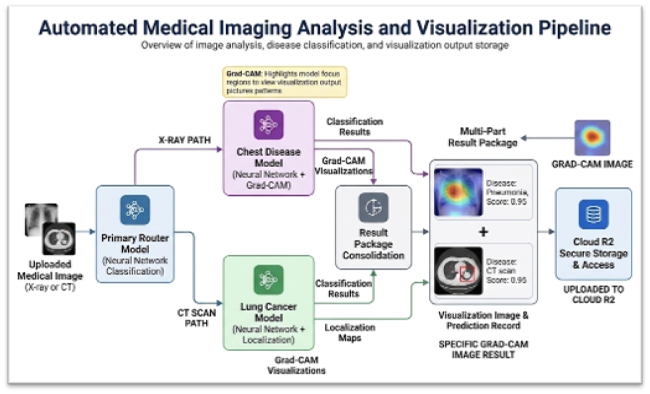
\includegraphics[width=0.95\linewidth]{assets/backend17.png}
	\caption{A simple visualization of the overall image processing pipeline from the backend's perspective.}
	\label{fig:backend_overall}
\end{figure}

\subsubsection{Grad-CAM Explainability and Localization}
For every chest X-ray prediction, the system generates a Grad-CAM (Gradient-weighted Class Activation Mapping) heatmap to provide interpretability for the AI decision. This mechanism highlights the regions of the image that most influenced the model’s prediction by tracing gradients flowing into the final convolutional layers of the DenseNet network.

The generated heatmap is visualized using a JET colormap and overlaid on the original X-ray image , allowing both the anatomical structure and the activated regions to remain clearly visible. This overlay helps radiologists and clinicians visually verify whether the model is focusing on medically relevant areas such as lung opacities, consolidations, or abnormal tissue patterns rather than irrelevant regions.

To support persistence and later retrieval, both the original Grad-CAM output and the processed overlay image are stored in Cloudflare R2 under the \texttt{heatmaps/} directory. These images are served to the frontend using secure presigned URLs, ensuring controlled and time-limited access to sensitive medical data.

\subsubsection{Localization Capability}Beyond explainability, Grad-CAM also provides a form of weak localization for disease regions within the chest X-ray. Although the DenseNet model is primarily designed for classification, Grad-CAM transforms it into a pseudo-localization system by identifying spatial regions that contribute most strongly to the predicted class.

This allows the system to:
\begin{itemize}
	\item Approximate the location of abnormal lung regions.
	\item Highlight areas associated with diseases.
	\item Provide spatial context without requiring a dedicated detection model   
\end{itemize}

In practice, this means the system not only predicts the presence of a disease but also indicates where in the lungs the abnormality is likely located. This improves clinical trust and makes the AI output more interpretable, bridging the gap between pure classification models and spatially aware diagnostic tools.

Overall, Grad-CAM serves as both an explainability mechanism and a lightweight localization method, enhancing transparency and clinical usability of the AI predictions.

\subsubsection{RAG Chatbot Module}
Retrieval-Augmented Generation (RAG) is an AI technique that enhances LLM responses by grounding them in a private document corpus rather than relying solely on the model's pre-trained knowledge. This is critical for domain-specific applications — such as medical systems,  where accuracy, traceability, and up-to-date information are essential.

\paragraph{Standard RAG Pipeline}
\begin{itemize}
	\item Ingest:  Load source documents (PDF, TXT, etc.)
	\item Chunk: Split long documents into overlapping smaller pieces.
	\item Embed: Convert each chunk to a dense numerical vector using a sentence embedding model.
	\item Store: Persist vectors in a FAISS vector database, organized by category.
	\item Retrieve: On a user query, embed the question and find the top-k most similar chunks.
	\item Generate: Pass the retrieved chunks and the question to the LLM to produce a grounded answer.
\end{itemize}

The classifier is the key differentiator of this RAG system. Rather than searching all documents indiscriminately, each query is first categorized, enabling targeted retrieval from the correct FAISS index.

\paragraph{Categories}
\begin{table}[htbp]
	\centering
	\caption{Categories of input handled by the RAG-based medical chatbot.}
	\label{tab:rag_input_categories}
	\begin{tabular}{|p{4cm}|p{9cm}|}
		\hline
		\textbf{Category} & \textbf{Typical Content} \\
		\hline
		
		Medical &
		Queries related to chest diseases and lung cancer, including symptoms, diagnosis, interpretation of medical findings, and general medical imaging questions. \\
		\hline
		
		General &
		Greetings, small talk, and off-topic or non-medical conversational queries that do not require clinical or diagnostic knowledge. \\
		\hline
		
	\end{tabular}
\end{table}

\paragraph{Model Architecture}
The classifier uses a lightweight 1D Convolutional Neural Network (CNN) designed for speed and bilingual text support, the full visualization of the architecture is shown in Figure~\ref{fig:rag_arch}.
\begin{enumerate}
	\item Input: Token IDs (max 50 tokens)
	\item Embedding Layer (vocab $\rightarrow$ 64 dims)
	\item Conv1d (64 $\rightarrow$ 128 channels) + ReLU + Dropout(0.3)
	\item Conv1d (128 $\rightarrow$ 128 channels) + ReLU
	\item AdaptiveMaxPool1d(1)
	\item Fully Connected: 128 $\rightarrow$ 64 $\rightarrow$ 3
	\item Output.
\end{enumerate}

\begin{figure}[htbp]
	\centering
	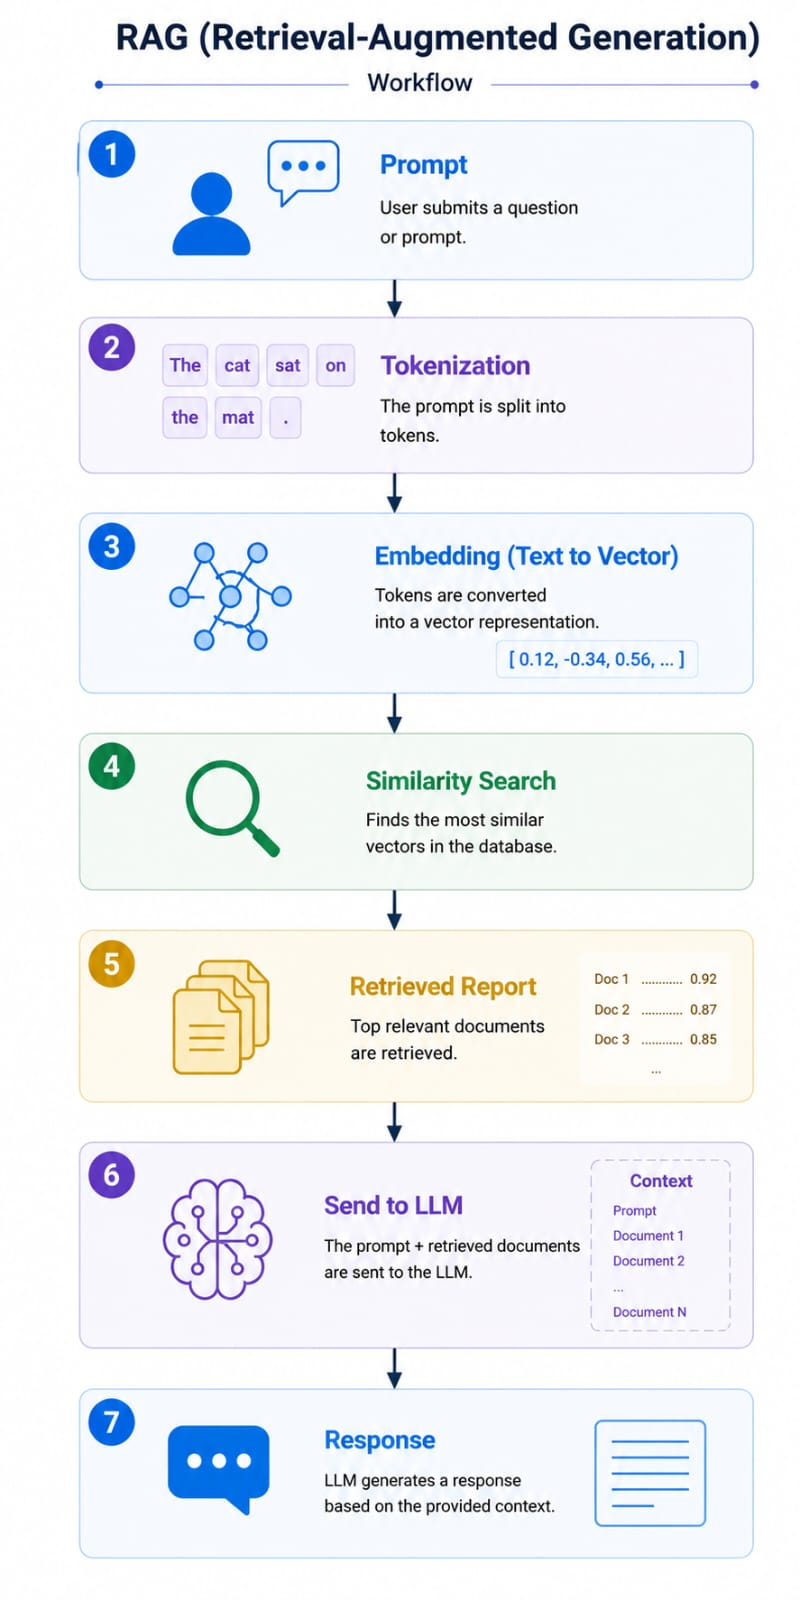
\includegraphics[height=0.90\textheight, keepaspectratio]{assets/backend18.jpeg}
	\caption{A simple visualization of the overall RAG architecture.}
	\label{fig:rag_arch}
\end{figure}

\paragraph{Bilingual Tokenizer}
\begin{itemize}
	\item Tokenizes Arabic , English, and numeric tokens
	\item Vocabulary built from training data (~300+ labeled question pairs)
	\item Fixed-length encoding: max 50 tokens, padded with <PAD>, unknown words as <UNK>
	\item Outputs: classifier.pth, tokenizer.json, config.json
\end{itemize}

\paragraph{Training Configuration}
The model was trained for 100 epochs using the Adam optimizer with a learning rate of 0.001 and a batch size of 16. The vocabulary size is 352 tokens, and each input token is mapped into a 64-dimensional embedding space. The hidden layer dimension is set to 128, Each input sequence is limited to a maximum length of 50 tokens to ensure consistent processing and performance.

\paragraph{LLM Configuration}
The configurations used for the RAG engine are shown in Table~\ref{tab:llm_parameters} for reproduce-ability purposes.
\begin{table}[htbp]
	\centering
	\caption{Configuration parameters of the RAG-based LLM engine.}
	\label{tab:llm_parameters}
	\begin{tabular}{|p{5cm}|p{8cm}|}
		\hline
		\textbf{Parameter} & \textbf{Standalone Value} \\
		\hline
		
		LLM Engine &
		Ollama \\
		\hline
		
		Model &
		qwen2.5:3b \\
		\hline
		
		Temperature &
		0.5 \\
		\hline
		
		Max Tokens &
		500 \\
		\hline
		
		Keep Alive &
		Infinite (-1) \\
		\hline
		
	\end{tabular}
\end{table}

\paragraph{Prompt Design}
The LLM is strictly instructed to answer only from the retrieved context. If the context does not contain the answer, the model is instructed to say "I don't know." Responses are capped at three sentences and must match the language of the question.

The text is split using a RecursiveCharacterTextSplitter with a chunk size of 1000 characters and an overlap of 150 characters between consecutive chunks. This ensures that the text is broken into manageable segments while preserving context between adjacent chunks for better retrieval accuracy.

RAG Independence from Image models  RAG does not receive chest X-ray predictions, GradCAM heatmaps, lung cancer results, or Spring Boot patient records. It is a standalone medical Q\&A chatbot co-located in every page  purely for deployment convenience.

Examples of using the RAG agent implemented in the system are shown in Figure~\ref{fig:rag_examples}

\begin{figure}[htbp]
	\centering
	
	% ---------------- Left Example ----------------
	\begin{subfigure}[t]{0.48\textwidth}
		\centering
		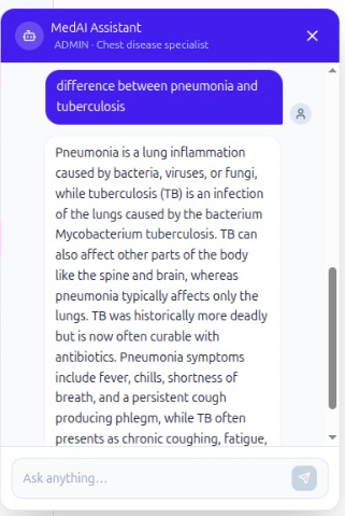
\includegraphics[width=\linewidth]{assets/backend19.png}
		\caption{Example of a medical query processed by the RAG agent, showing retrieval of relevant documents and generated response.}
		\label{fig:rag_example_1}
	\end{subfigure}
	\hfill
	% ---------------- Right Example ----------------
	\begin{subfigure}[t]{0.48\textwidth}
		\centering
		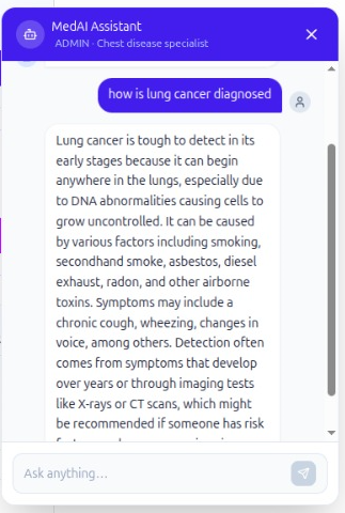
\includegraphics[width=\linewidth]{assets/backend20.png}
		\caption{Example of a general/off-topic query handled by the RAG agent with a conversational response without medical retrieval.}
		\label{fig:rag_example_2}
	\end{subfigure}
	
	\caption{Illustrative examples of the behavior of the retrieval-augmented generation (RAG) agent in different query scenarios. The system adapts its response strategy depending on whether the input is medical or general in nature.}
	\label{fig:rag_examples}
\end{figure}


\subsubsection{Performance Profile}
The performance profile of the proposed system is discussed in Table~\ref{tab:performance_overview}.
\begin{table}[htbp]
	\centering
	\caption{Computational performance and execution environment of the proposed system components.}
	\label{tab:performance_overview}
	\begin{tabular}{|p{5cm}|p{4cm}|p{5cm}|}
		\hline
		\textbf{Component} & \textbf{Approximate CPU Time} & \textbf{GPU} \\
		\hline
		
		Router &
		50--100 ms &
		Automatically enabled if CUDA is available \\
		\hline
		
		Chest Pipeline (Segmentation + Prediction + Grad-CAM) &
		1--5 s &
		CUDA auto-enabled \\
		\hline
		
		Lung Cancer YOLO Inference &
		1--5 s &
		CUDA auto-enabled \\
		\hline
		
		R2 Download / Upload &
		Network-dependent &
		N/A \\
		\hline
		
	\end{tabular}
\end{table}

Running the ModelBackend requires sufficient computational resources because it hosts multiple AI components simultaneously, including image classification models (DenseNet, YOLO, U-Net), the router model, and the RAG pipeline with embedding models and an LLM (Ollama). For stable performance, a GPU is strongly recommended for accelerating deep learning inference, especially for chest X-ray and lung cancer detection tasks.

In addition, the system requires adequate CPU resources to handle concurrent API requests, image preprocessing, and routing logic, while RAM (at least 4–6 GB minimum, higher recommended) is needed to keep multiple models, FAISS indexes, and embeddings loaded in memory without performance degradation. Overall, a balanced setup with a capable GPU, multi-core CPU, and sufficient RAM ensures smooth and responsive AI processing across all services in the ModelBackend

\subsection{Federated Learning Server}
The Federated-Learning-Server is responsible for enabling privacy-preserving collaborative training across multiple hospitals without requiring any centralization of medical data. It allows hospitals to jointly train a shared model while ensuring that raw patient images never leave their local environments, maintaining strict data privacy and compliance with healthcare constraints.

The system is built using a hybrid architecture that combines a FastAPI REST service and a Flower-based gRPC server within a single Python process. The FastAPI layer acts as the control interface for registration, monitoring, and coordination tasks, while the Flower server handles the actual federated learning workflow, including distributed training and weight aggregation.

Both components are synchronized through an in-memory SharedState singleton, which maintains the current training status, active clients, and round coordination signals. This design allows seamless communication between REST-based administrative actions and gRPC-based training execution, ensuring that federated learning rounds are executed in a coordinated and efficient manner across all participating hospitals.

\subsubsection{Design Principles}
The design principles of the federated learning server are listed in Table~\ref{tab:fl_principles}.
\begin{table}[htbp]
	\centering
	\caption{Core design principles and their implementation in the federated learning framework.}
	\label{tab:fl_principles}
	\begin{tabular}{|p{4cm}|p{9cm}|}
		\hline
		\textbf{Principle} & \textbf{Implementation} \\
		\hline
		
		Privacy first &
		Only model weight updates are transmitted between clients and the server; raw medical images never leave the hospital premises under any circumstance. \\
		\hline
		
		On-demand training &
		The Flower server remains idle until explicitly triggered by an administrator via the \texttt{POST /start-round} endpoint, ensuring that training rounds are fully controlled and non-automatic. \\
		\hline
		
		In-process coupling &
		FastAPI and Flower operate within a shared runtime environment using a \texttt{SharedState} singleton, eliminating the need for internal HTTP communication and reducing overhead. \\
		\hline
		
		Weight hot-reload &
		After each federated aggregation round, the updated global model weights are immediately pushed to the Model Backend, enabling real-time deployment of improved models. \\
		\hline
		
	\end{tabular}
\end{table}

The Federated-Learning-Server follows a dual-process architecture where two interconnected services run simultaneously within the same system. The main process runs a Uvicorn-based FastAPI server on port 8001, which acts as the REST bridge responsible for hospital registration, client management, monitoring, and handling webhooks from the main backend system. In parallel, a daemon process runs a Flower gRPC server on port 50051, which is responsible for coordinating the actual federated learning workflow, including distributed training and model weight aggregation across participating hospitals.

This separation allows the system to clearly divide responsibilities between control-plane operations (handled by FastAPI) and training-plane execution (handled by Flower). Both processes share a common in-memory SharedState, ensuring synchronization between REST actions and federated learning events while maintaining efficient and real-time coordination.

\subsubsection{Training Round Lifecycle}
A complete federated training round follows these steps:
\begin{itemize}
	\item Step 1: Admin selects online hospitals and initiates a round
	\item Step 2: Spring calls start-round with round id, min clients, deadline minutes
	\item Step 3: FastAPI sets SharedState \texttt{trigger\_event}, unblocking the Flower server thread
	\item Step 4: Hospital clients receive global weights via gRPC, train locally on their data
	\item Step 5: CustomFedAvg aggregates weight updates using the FedAvg algorithm
	\item Step 6: Aggregated weights saved and pushed to ModelBackend
	\item Step 7: Webhook notifies spring of round completion or failure
	\item Step 8: trigger event cleared; Flower waits for the next admin trigger
\end{itemize}

\begin{figure}[htbp]
\centering
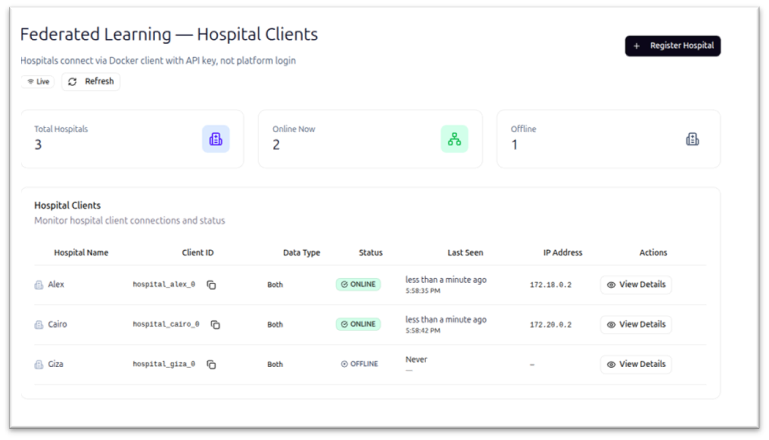
\includegraphics[width=0.95\linewidth]{assets/backend21.png}
\caption{The federated learning dashboard of the web application.}
\label{fig:fed_db}
\end{figure}

After a hospital is successfully registered in the federated learning system, Spring Boot finalizes the onboarding process by generating the necessary FL credentials and preparing a deployment package for that hospital. Once the registration is approved, the system automatically sends an email notification to the hospital using Gmail SMTP.

This email contains all essential onboarding information, including the hospital’s federated learning client ID, encrypted API key, and instructions for connecting to the Federated Learning Server. It also provides a Docker-based hospital client package, which is the only component the hospital needs to run locally.

From the hospital side, the setup process is intentionally simple. The hospital team only needs to:
\begin{enumerate}
	\item Put the data in the required folder
	\item Run the container provided in the package 
\end{enumerate}

Once the container is started, the hospital client automatically connects to the Federated Learning Server, begins sending heartbeat signals, and becomes eligible for participation in training rounds. After this step, no further manual integration is required, as all communication and training coordination are handled automatically by the system.

This design ensures a smooth onboarding process where hospitals do not need to manage complex machine learning setups, and can join the federated learning network by simply configuring and running a pre-built container

Once the container is running and sending heartbeat signals, the hospital is marked as ONLINE and becomes eligible to participate in federated training rounds.

\begin{figure}[htbp]
	\centering
	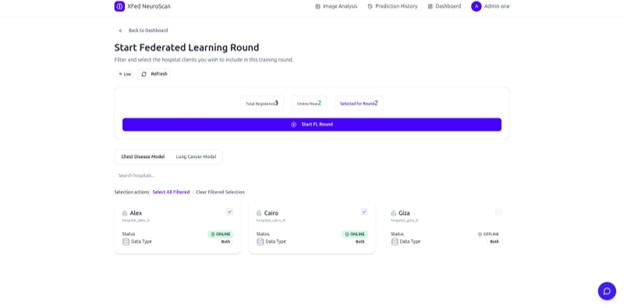
\includegraphics[width=0.95\linewidth]{assets/backend22.jpg}
	\caption{The federated learning management tab.}
	\label{fig:fed_mgmt}
\end{figure}

\subsubsection{Round Status States}
The full states and status code for the federated learning server are listed and explained in Table~\ref{tab:fl_status}
\begin{table}[htbp]
	\centering
	\caption{Federated learning server execution states and their meanings.}
	\label{tab:fl_status}
	\begin{tabular}{|p{3.5cm}|p{10cm}|}
		\hline
		\textbf{Status} & \textbf{Meaning} \\
		\hline
		
		IDLE &
		No federated learning round is currently running; the Flower server is blocked and waiting for an external trigger event. \\
		\hline
		
		STARTED &
		A training round has been triggered and participating hospital clients are actively performing local model training. \\
		\hline
		
		AGGREGATING &
		The server is performing FedAvg aggregation over received client updates to compute the new global model. \\
		\hline
		
		COMPLETED &
		The federated learning round has successfully finished, and the updated global model weights have been saved and pushed to the Model Backend for deployment. \\
		\hline
		
		FAILED &
		The federated learning round has failed due to issues such as timeouts, client-side errors, or model update push failures. \\
		\hline
		
	\end{tabular}
\end{table}

\subsubsection{Security}
The Federated Learning security model is designed to ensure strict isolation between hospitals, the platform backend, and the training infrastructure. A Platform API key is used exclusively by the centralized Backend to securely register new hospital clients, retrieve client lists, and initiate federated learning rounds, ensuring that only the trusted backend can control system-level operations.

Each hospital node is assigned a unique Client API key, which is used solely for heartbeat authentication to confirm that the hospital is online and eligible to participate in training. In addition, a Webhook secret is shared between the FL Server and centralized  Backend to verify and secure all outbound callbacks related to training round completion and status updates.

Hospitals communicate with the system only through outbound connections to port 8001 for REST heartbeats and port 50051 for gRPC-based training, eliminating the need for direct inbound access. Importantly, admin users never interact directly with the FL Server; instead, all operations are securely routed through centralized Backend using JWT authentication, maintaining a centralized and controlled security layer.

The various key types and their roles are shown and explained in great detail in Table~\ref{tab:fl_keys}.

\begin{table}[htbp]
	\centering
	\caption{Authentication key types and their roles within the federated learning system.}
	\label{tab:fl_keys}
	\begin{tabular}{|p{4cm}|p{4.5cm}|p{6cm}|}
		\hline
		\textbf{Key Type} & \textbf{Holder} & \textbf{Scope} \\
		\hline
		
		Platform API Key &
		Centralized Backend &
		Used by the backend system to register clients, initiate federated learning rounds, and retrieve the list of participating clients. \\
		\hline
		
		Client API Key &
		Each hospital node &
		Used exclusively for heartbeat authentication to verify active participation and connectivity of hospital clients. \\
		\hline
		
		Webhook Secret &
		Federated Learning Server and Centralized Backend &
		Used to authenticate outbound callback requests from the federated learning server after training rounds to ensure secure communication. \\
		\hline
		
	\end{tabular}
\end{table}

\subsection{End-to-End Data Flows}
\subsubsection{Medical Image Analysis Flow}
\begin{enumerate}
	\item The frontend user selects an image and requests a presigned URL from the Spring Backend.
	
	\item The frontend uploads the image directly to Cloudflare R2 using the provided presigned URL.
	
	\item After upload, the frontend calls the image processing service with the stored R2 key.
	
	\item The Spring Backend saves image metadata in PostgreSQL, generates a presigned URL, and forwards the request to the FastAPI service via Feign client communication.
	
	\item The FastAPI service downloads the image from R2, routes it using the trained routing model, and executes the appropriate specialist pipeline (either chest disease classification or lung cancer detection).
	
	\item The FastAPI service uploads the generated outputs (such as Grad-CAM heatmaps or annotated detection images) back to R2 and returns the prediction, confidence score, and storage key.
	
	\item The Spring Backend stores the final inference results in the database and generates presigned URLs for secure result visualization.
	
	\item The frontend displays the prediction results, confidence scores, and visual explanations such as Grad-CAM overlays or bounding box annotations to the user.
\end{enumerate}

\subsubsection{User Authentication Flow}
\begin{enumerate}
	\item The user logs in via the login page, where credentials are verified by Spring Security.
	
	\item If authentication succeeds, an access JWT is returned in the response body, and a refresh token is set as an HttpOnly cookie.
	
	\item The refresh token is also stored in Redis with a defined key and a 30-day expiration period.
	
	\item The frontend stores the access token in memory, while the authentication context initializes and loads the user role and profile information.
	
	\item When the access token expires, the frontend calls the refresh token endpoint, which issues a new access token and rotates the refresh cookie.
	
	\item During logout, the access token is blacklisted and the refresh token is removed from Redis, fully invalidating the user session.
\end{enumerate}

\subsubsection{Federated Learning Hospital Status Flow}
\begin{enumerate}
	\item The administrator registers a hospital through the frontend interface, and the Spring forwards the registration request to the Federated Learning (FL) Server.
	
	\item The FL Server generates a unique API key, which is encrypted and stored by the backend. Subsequently, an onboarding email containing the Docker-based client package is sent to the hospital.
	
	\item The hospital deploys the provided Docker client, which establishes a connection to the Flower server via gRPC for federated learning participation.
	
	\item The hospital client initiates a heartbeat process that continuously sends periodic signals to the FL Server every 30 seconds to indicate active status.
	
	\item The Spring Backend executes a polling mechanism every 10 seconds to retrieve the latest client status updates from the FL Server.
	
	\item The retrieved client statuses are synchronized with the PostgreSQL database and broadcast in real time using STOMP WebSocket communication.
	
	\item The frontend subscribes to the WebSocket channel and dynamically updates hospital ONLINE/OFFLINE indicators in real time based on received status updates.
\end{enumerate}